\documentclass[svgnames]{beamer}
\usepackage{graphicx}
\usepackage{amsmath}
\usepackage{hyperref}
\usepackage{booktabs}
\usepackage{multirow}
\usepackage{changepage}
\usepackage{subfig}
\usepackage{threeparttable}
\usepackage{bbm}
\usepackage{soul}
\usepackage{verbatim}
\usepackage{import}
\usepackage{bibentry}
\ifxetex
  \usepackage{fontspec}
\else
  \usepackage[T1]{fontenc}
  \usepackage[utf8]{inputenc}
  \usepackage{lmodern}
\fi

\setbeamercovered{transparent}

\hypersetup{
  colorlinks=true,
  citecolor=blue
}
\usepackage[round]{natbib}
\usetheme{Singapore}
\usecolortheme{rose}
\begin{document}

\begin{frame}
\title{Income Inequality and Health Inequality}
\author{Wenlan Luo}
\date{1/22/2015}
\maketitle
\end{frame}

\begin{frame}{Survival probability}
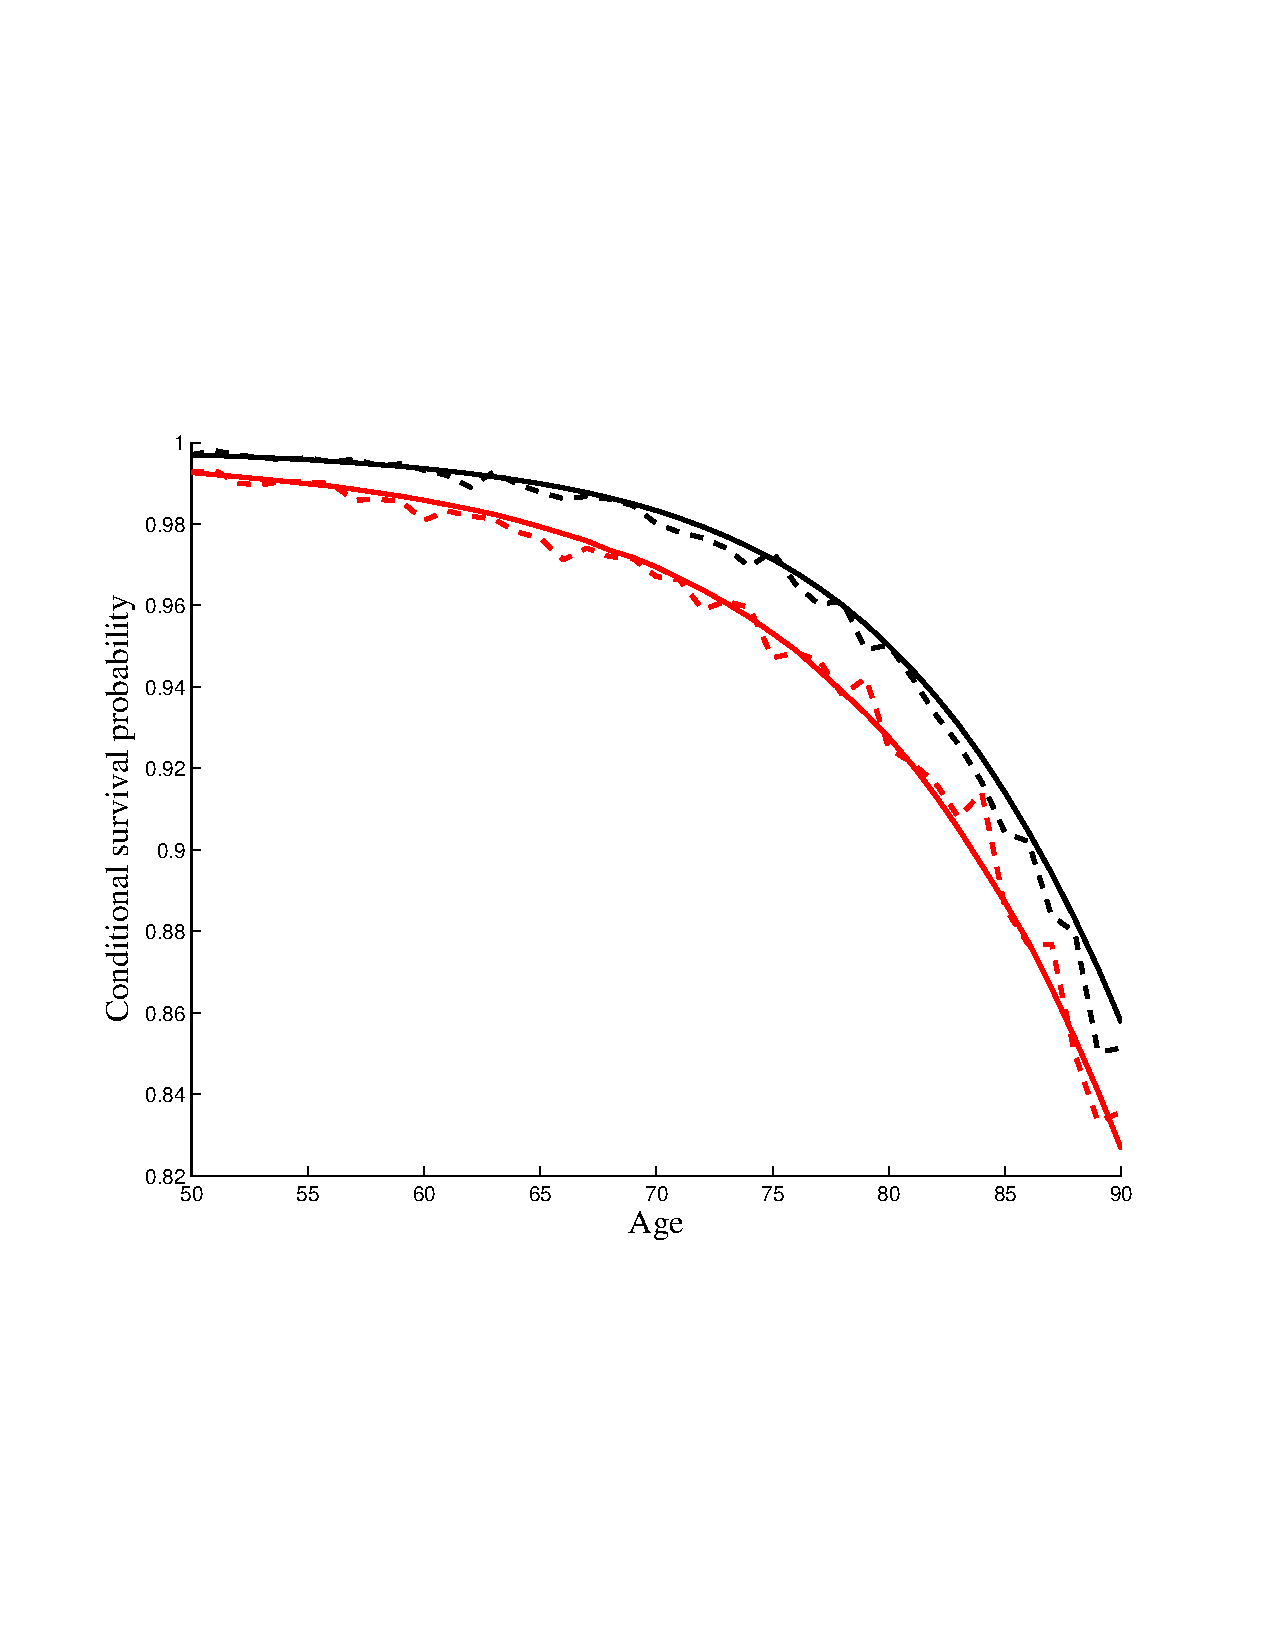
\includegraphics[width=1\textwidth, trim=0cm 0cm 0cm 5cm, clip=true]{graph/PsiModelVsData.pdf}
\end{frame}

\begin{frame}{Medical expenditure}
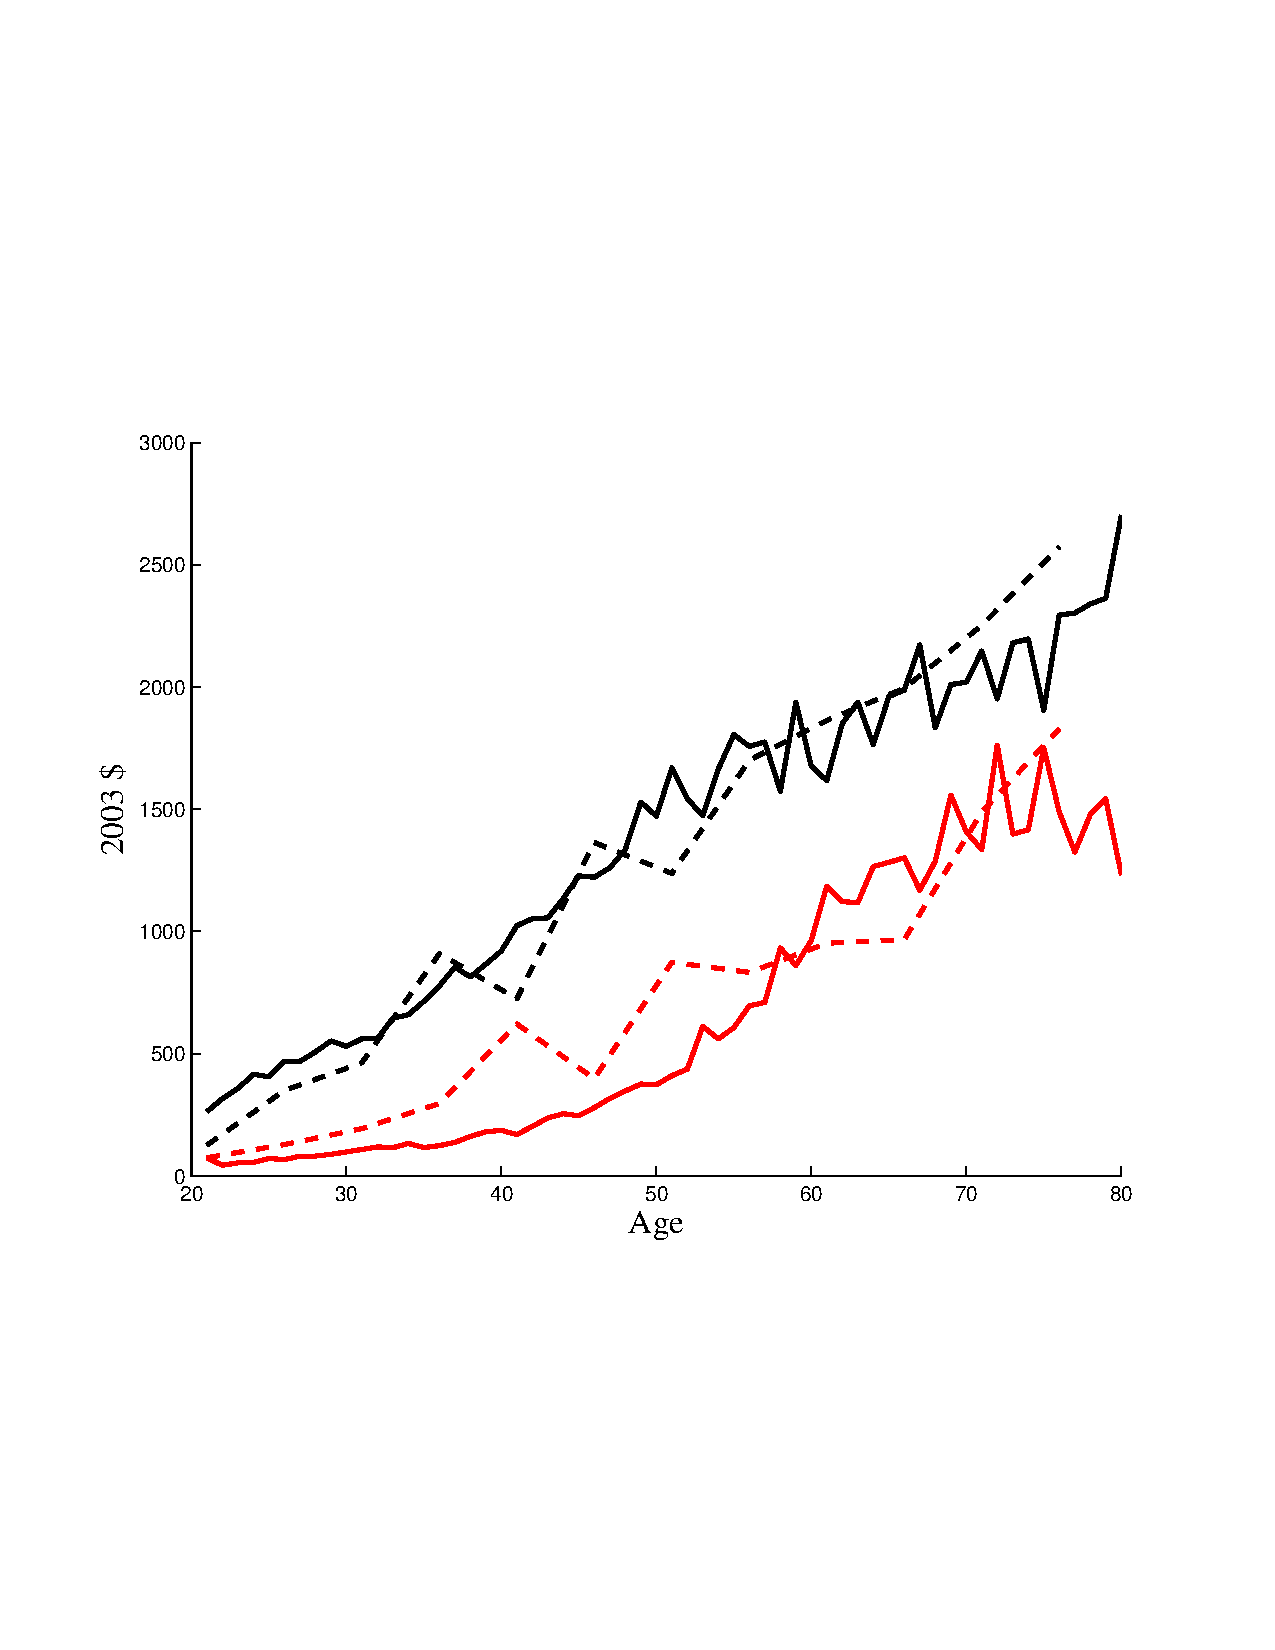
\includegraphics[width=1\textwidth, trim=0cm 0cm 0cm 5cm, clip=true]{graph/MedicalModelVsData.pdf}
\end{frame}

\begin{frame}{Change of consumption inequality}
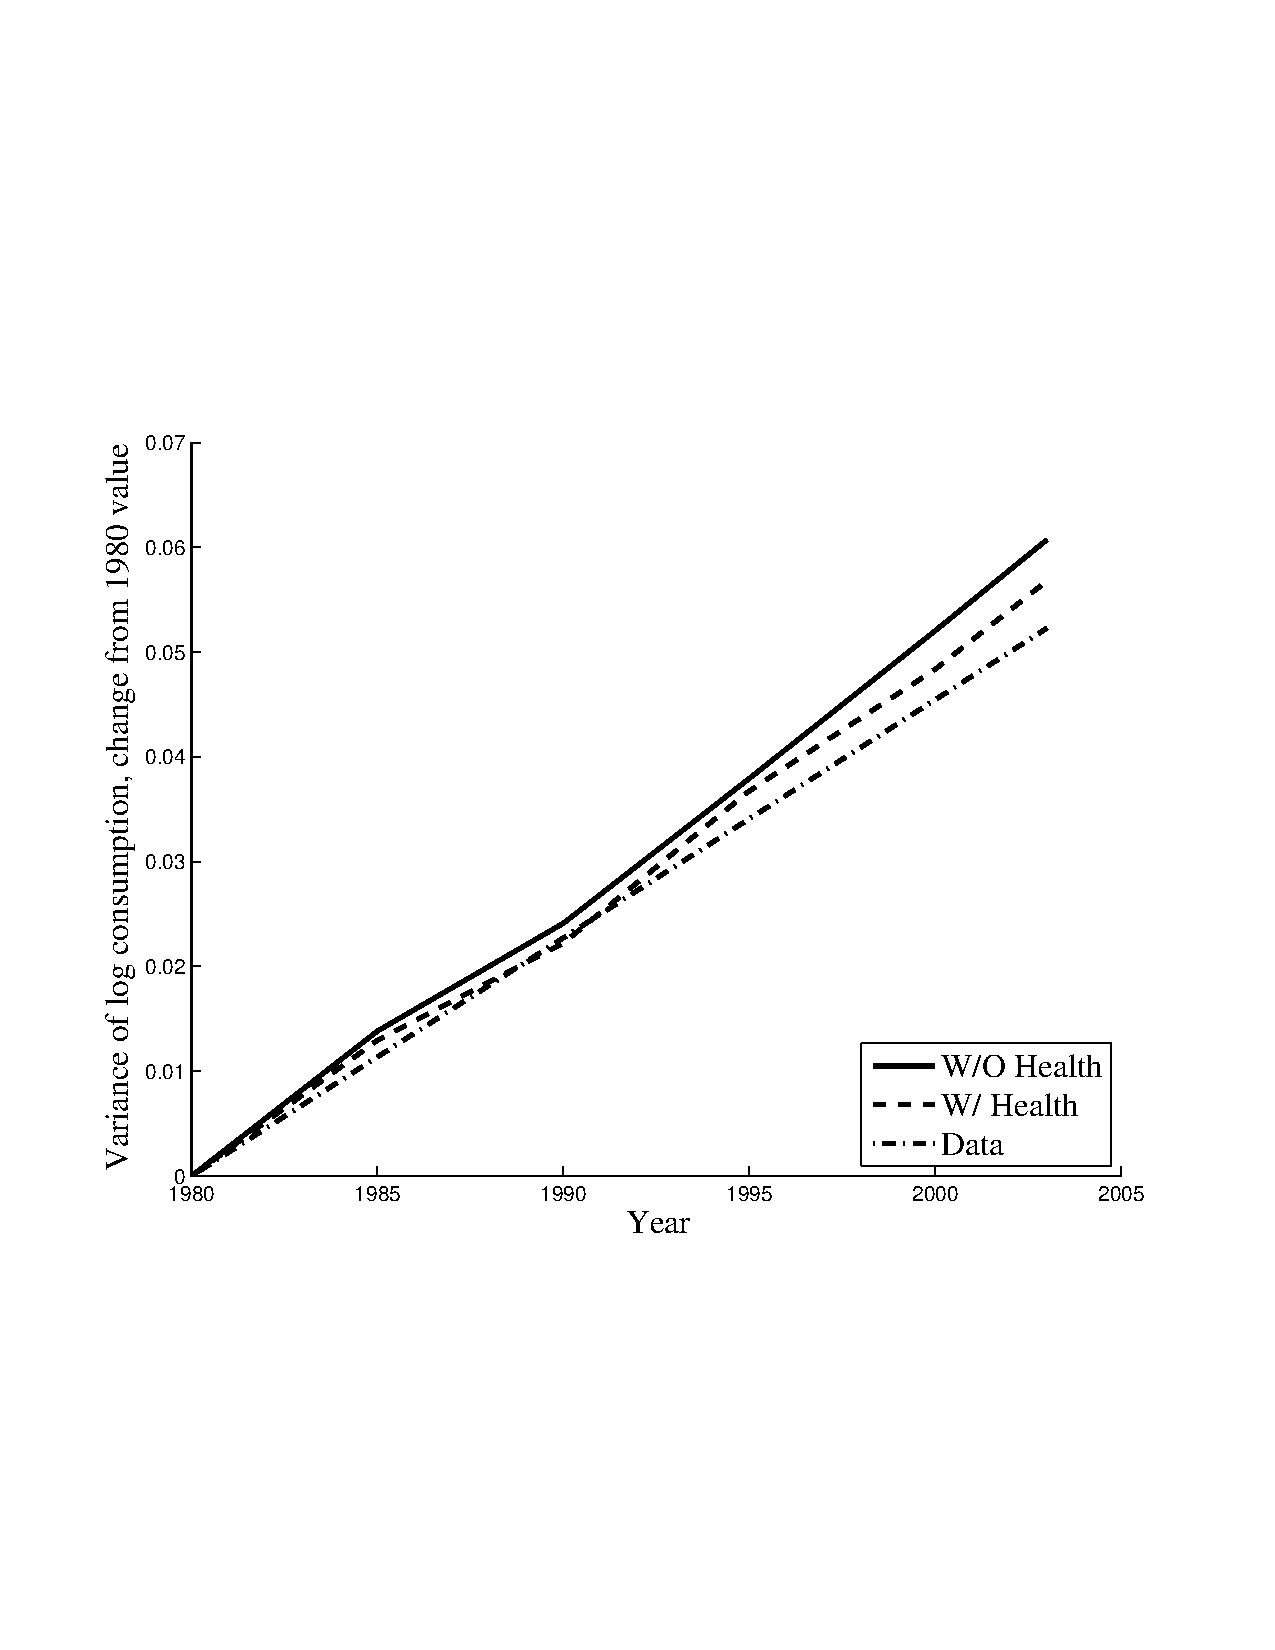
\includegraphics[width=1\textwidth, trim=0cm 0cm 0cm 5cm, clip=true]{graph/VarLogCByYear.pdf}
\end{frame}


\begin{frame}{Change of consumption inequality}
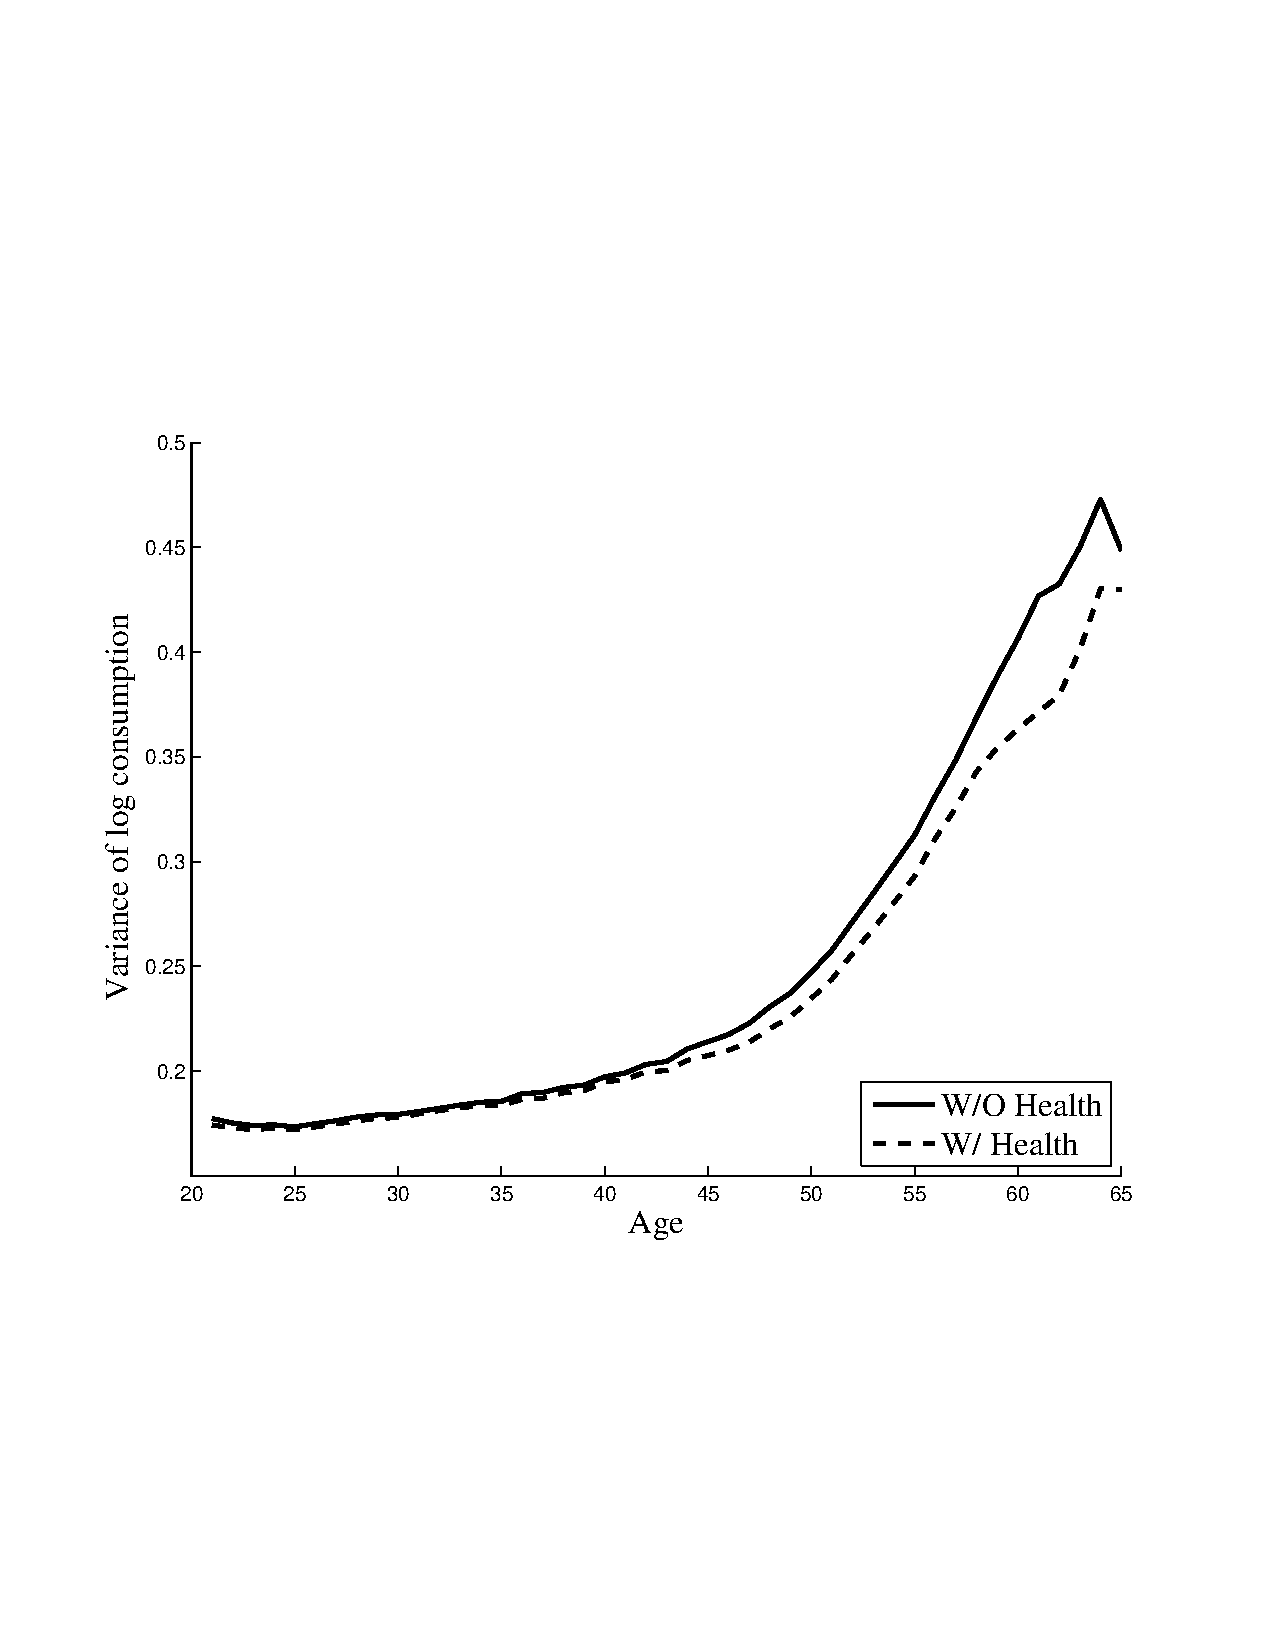
\includegraphics[width=1\textwidth, trim=0cm 0cm 0cm 5cm, clip=true]{graph/VarLogCByAge.pdf}
\end{frame}


\end{document}